% https://mirrors.ibiblio.org/CTAN/fonts/fontawesome/doc/fontawesome.pdf
\documentclass[a4paper,12pt, final]{article}
% Adjust the page margins if needed
% \usepackage[scale=0.75]{geometric}
% \usepackage[utf8]{inputenc}
\usepackage[english]{babel}
\usepackage[
    ignoreheadfoot, % set margins without considering header and footer
    top=2cm, % separation between body and page edge from the top
    bottom=3cm, % separation between body and page edge from the bottom
    left=2cm, % separation between body and page edge from the left
    right=2cm, % separation between body and page edge from the right
    footskip=1.5cm, % separation between body and footer
]{geometry} % for adjusting page geometry
\usepackage{float}

\usepackage[explicit]{titlesec} % for customizing section titles
% \usepackage{tabularx} % for making tables with fixed width columns
% \usepackage{array} % tabularx requires this
% \usepackage[dvipsnames]{xcolor} % for coloring text
% \definecolor{primaryColor}{RGB}{0, 79, 144} % define primary color
% \definecolor{primaryColor}{RGB}{0, 0, 0} % define primary color
\usepackage{enumitem} % for customizing lists
% \usepackage{fontawesome5} % for using icons
\usepackage{amsmath} % for math
\usepackage[
    pdftitle={},
    pdfauthor={},
    % colorlinks=true,
    % urlcolor=primaryColor
]{hyperref} % for links, metadata and bookmarks
% \usepackage[pscoord]{eso-pic} % for floating text on the page
% \usepackage{calc} % for calculating lengths
% \usepackage{bookmark} % for bookmarks
\usepackage{lastpage} % for getting the total number of pages
\usepackage[default, type1]{sourcesanspro} % for using source sans 3 font
% \usepackage{ifthen}
\usepackage{fancyhdr}
\usepackage{graphicx}
% \usepackage{blindtext}

% Team Information
\newcommand{\ourteam}{}

\title{EcoRoute}
% % % Header and Footer Styling
% Some settings:
\pagestyle{empty} % no header or footer
\pagestyle{fancy}
\fancyhf{} % sets both header and footer to nothing
\renewcommand{\headrulewidth}{0pt}
\fancyfoot[CO,RE]{\color{gray}\textit{\small \ourteam \ - Page \thepage{} of \pageref*{LastPage}}}



% \titleformat{\section}{
%     % make the font size of the section title large and color it with the primary color
%     \Large\color{primaryColor}
% }{
% }{
% }{
%     % print bold title, give 0.15 cm space and draw a line of 0.8 pt thickness
%     % from the end of the title to the end of the body
%     \textbf{#1}\hspace{0.15cm}\titlerule[0.8pt]\hspace{-0.1cm}
% }[] % section title formatting

% \titlespacing{\section}{
%     % left space:
%     0pt
% }{
%     % top space:
%     0.3 cm
% }{
%     % bottom space:
%     0.2 cm
% } % section title spacing

% \titleformat{\subsection}{
%     % \color{primaryColor}
% }{
% }{
% }{
%     #1 \hspace{0.15cm}\hspace{-0.1cm}
% }[] % section title formatting

% \newenvironment{header}{
%     \setlength{\topsep}{0pt}\par\kern\topsep\centering\color{primaryColor}\linespread{1.5}
% }{
%     \par\kern\topsep
% } % new environment for the header

\newcommand{\placelastupdatedtext}{% \placetextbox{<horizontal pos>}{<vertical pos>}{<stuff>}
    \AddToShipoutPictureFG*{% Add <stuff> to current page foreground
        \put(
        \LenToUnit{\paperwidth-2 cm-0.2 cm+0.05cm},
        \LenToUnit{\paperheight-1.0 cm}
        ){\vtop{{\null}\makebox[0pt][c]{
                    % \small\color{gray}\textit{Last updated in February 2024}\hspace{\widthof{Last updated in February 2024}}
                    \small\color{gray}\textit{Last updated on \today}\hspace{\widthof{Last updated on \today}}
        }}}%
    }%
}%

% save the original href command in a new command:
\let\hrefWithoutArrow\href
% new command for external links:
\renewcommand{\href}[2]{\hrefWithoutArrow{#1}{\mbox{\ifthenelse{\equal{#2}{}}{ }{#2 }\raisebox{.15ex}{\footnotesize \faExternalLink*}}}}


% For TextEntrys (see https://tex.stackexchange.com/a/600/287984):
% \def\changemargin#1#2{\list{}{\rightmargin#2\leftmargin#1\topsep=0pt\itemsep=0pt\parsep=0pt\parskip=0pt\labelwidth=0pt\itemindent=0pt\labelsep=0pt}\item[]}
% \let\endchangemargin=\endlist 

% Ensure that generate pdf is machine readable/ATS parsable
\pdfgentounicode=1
% \pagestyle{customFooterStyle}



% Begin Document
\author{THAMER ALHARBI, Faisal Alshammari, Badr Alharbi}
\begin{document}
% \fancyfoot[R]{}
% \placelastupdatedtext
\maketitle
% % Title/Header
% \vspace{0.3 cm}

\tableofcontents
\listoffigures
\listoftables

\newpage
\section{Executive Summary}
This idea focuses on improving the delivery process by optimizing truck routes. The company is
currently facing high delivery costs due to inefficient truck routing.
The proposed solution involves using clustering techniques (DBSCAN or K-means) and solving the
Vehicle Routing Problem (VRP) to reduce delivery time and costs.

\section{Problem Statement}
The company is currently experiencing high logistics costs due to inefficient truck routing and
suboptimal customer clustering. This leads to increased delivery time and excessive fuel
consumption.

\section{Proposed Solution}
The solution relies on using clustering algorithms to group customers based on proximity and then
optimizing truck routes using Vehicle Routing Problem (VRP) algorithms. Trucks will be assigned
based on their capacity to maximize efficiency.

\subsection{Benefits of Solution}
\begin{enumerate}
    \item \textbf{Reduce Costs by Minimizing Fuel Consumption:} By optimizing routes and utilizing automated systems for loading and unloading, the solution reduces unnecessary travel and idle times, resulting in significant fuel savings. 
    \item \textbf{Improve Efficiency by Reducing Delivery Times:} By optimizing routes ensuring faster and more accurate service while enhancing overall operational efficiency.
    \item \textbf{Scalability:} The solution is designed to grow as the number of trucks and customers increases. Automation supports seamless scaling by maintaining high efficiency even as operational demands expand.
\end{enumerate}

\subsection{How It Works}
\begin{enumerate}
    \item Receive customer orders and validate them.
    \item Cluster customers geographically.
    \item Assign trucks based on capacity and volume of packages.
    \item Optimize truck routes using VRP solutions.
    \item Calculate the most efficient paths for each truck.
\end{enumerate}

\section{Implementation Plan}
\begin{enumerate}
    \item Pilot test the solution in a small region.
    \item Full-scale implementation across the logistics network.
    \item Provide training to staff on the new system.
\end{enumerate}



\newpage
\section{Diagrams}
\subsection{Database Diagrams}
% \blindtext

\begin{figure}[h]
   \centering
   \begin{tabular}{@{}c@{\hspace{.5cm}}c@{}}
       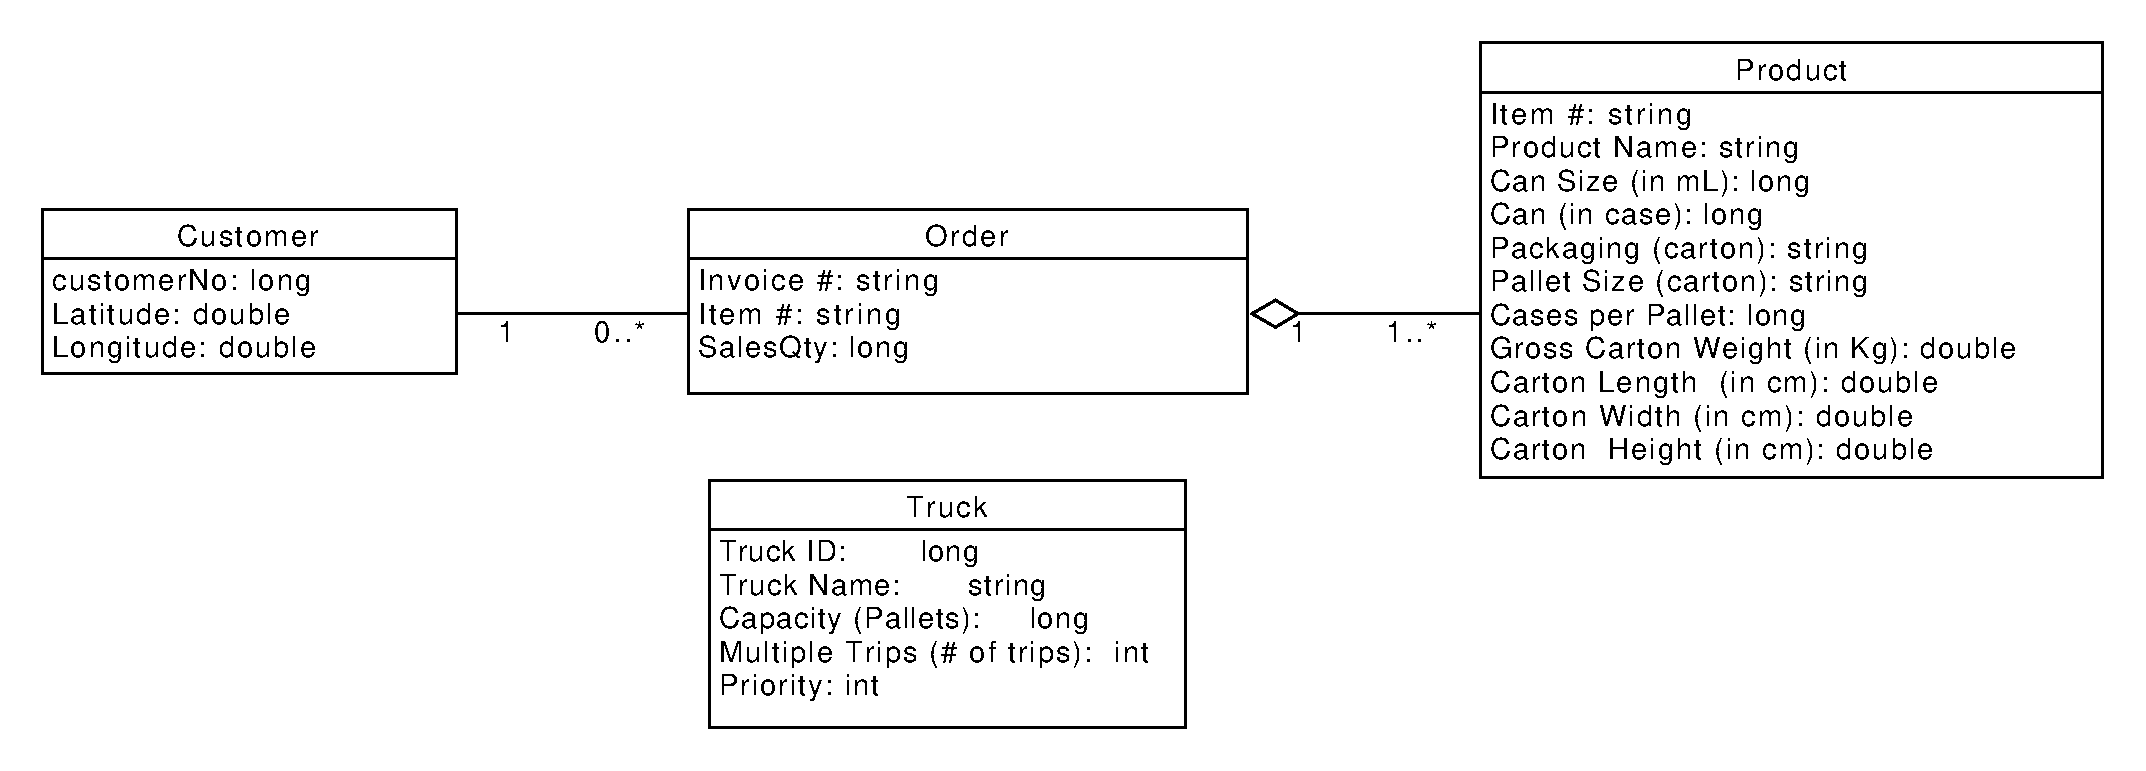
\includegraphics[page=1,width=1\textwidth]{gfx/TLDR_old_u.pdf}
       % \includegraphics[page=2,width=.45\textwidth]{somemultipagepdf} \\[.5cm]
       % \includegraphics[page=3,width=.45\textwidth]{somemultipagepdf} \\
   \end{tabular}
 \caption{Old Database Diagram}
 \label{fig:Test}
\end{figure}

% \blindtext

\begin{figure}[h]
   \centering
   \begin{tabular}{@{}c@{\hspace{.5cm}}c@{}}
       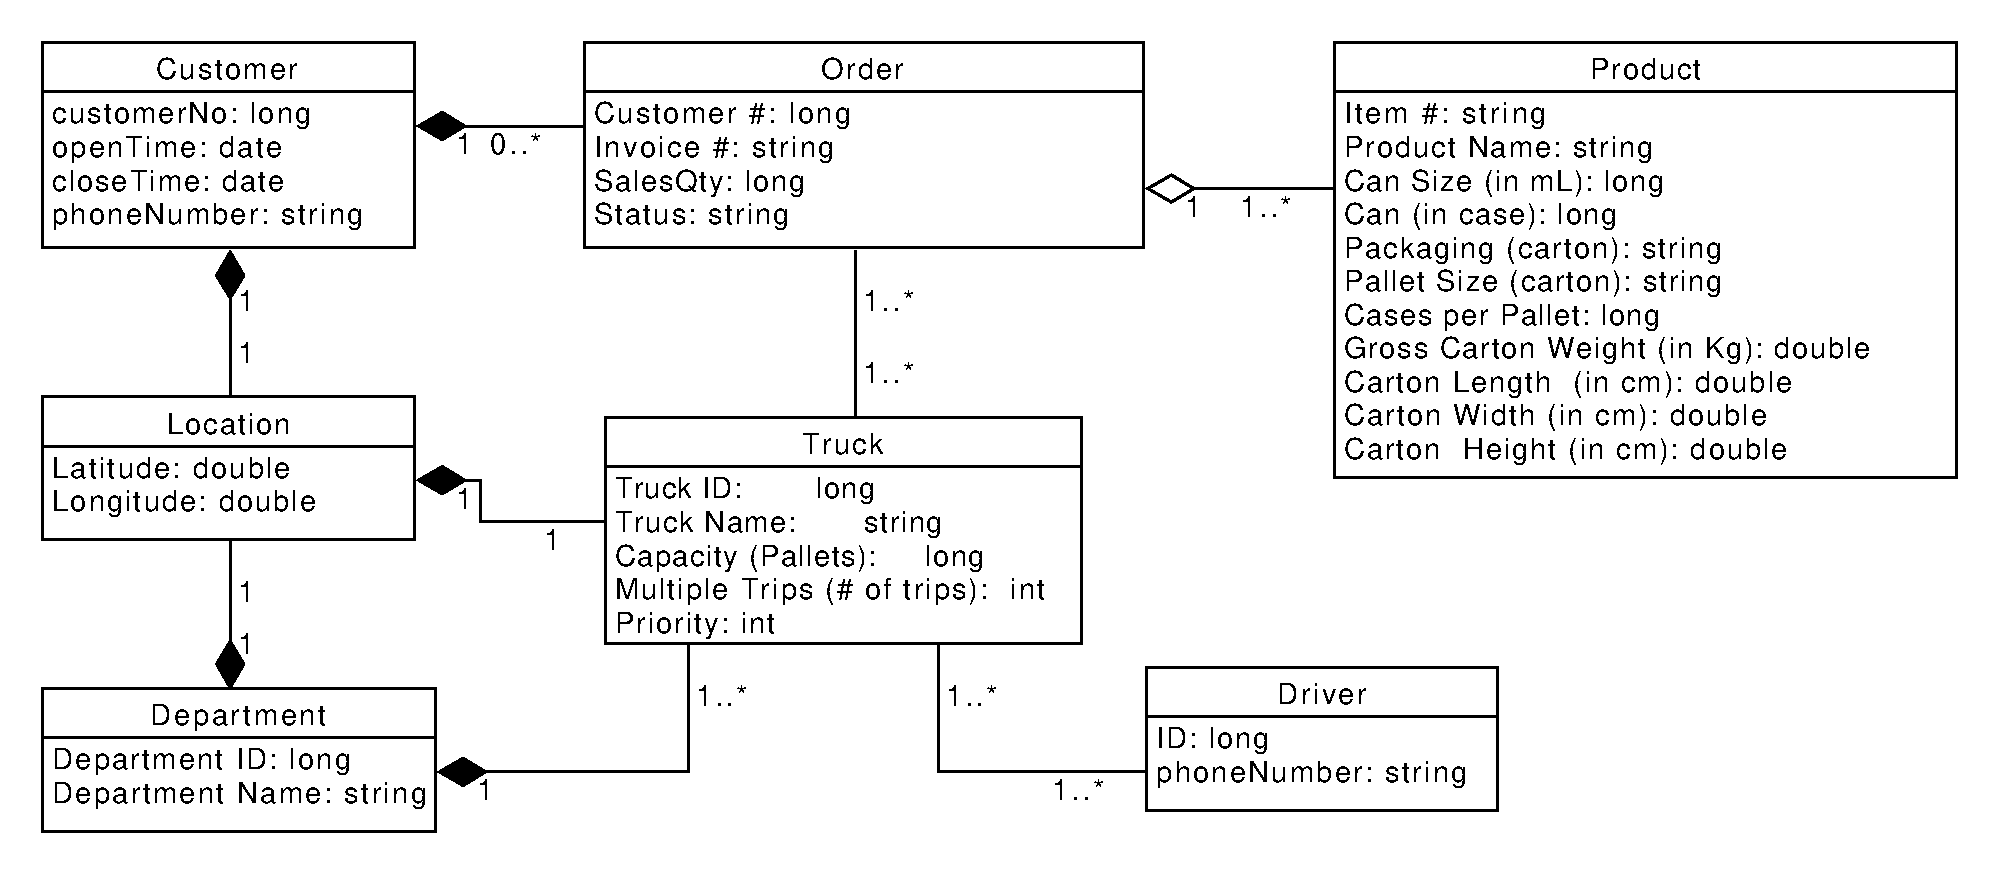
\includegraphics[page=1,width=1\textwidth]{gfx/TLDR_new_u.pdf} 
       % \includegraphics[page=2,width=.45\textwidth]{somemultipagepdf} \\[.5cm]
       % \includegraphics[page=3,width=.45\textwidth]{somemultipagepdf} \\
   \end{tabular}
 \caption{New Database Diagram}
 \label{fig:Test}
\end{figure}
\newpage
\subsection{Activity Diagrams}
\begin{figure}[h]
   \centering
   \begin{tabular}{@{}c@{\hspace{.5cm}}c@{}}
       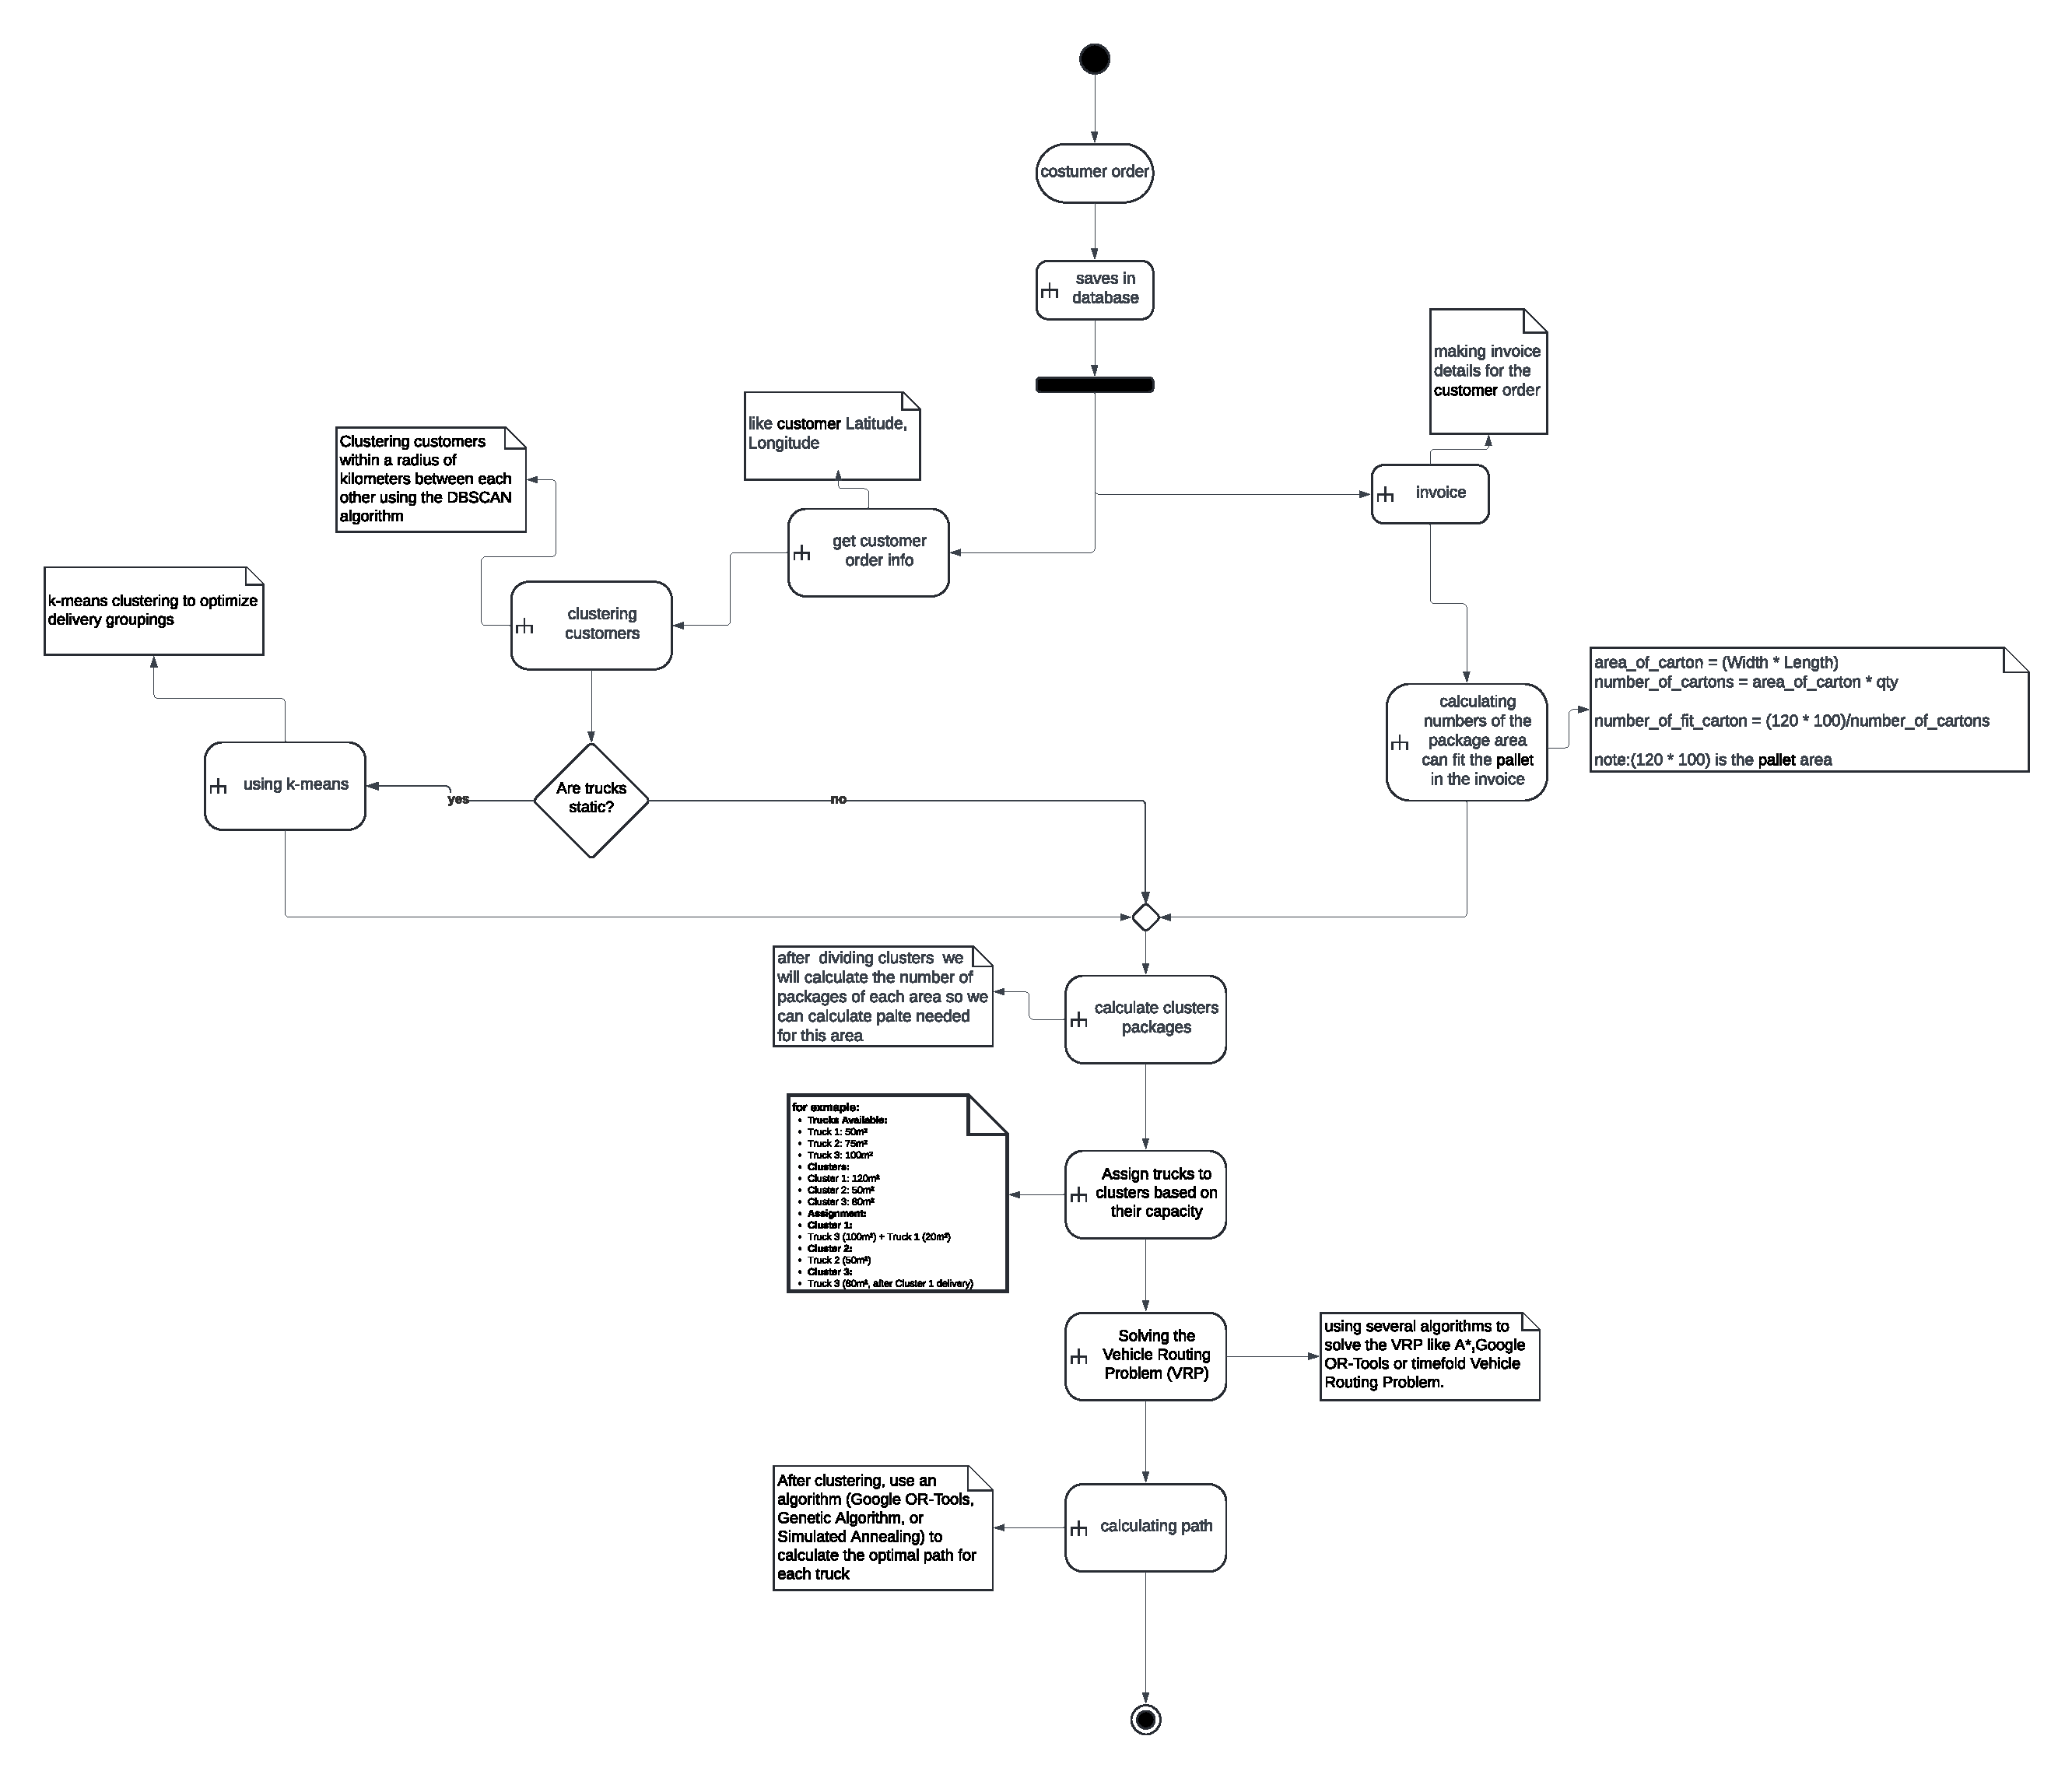
\includegraphics[page=1,width=1\textwidth]{gfx/TLDR_activity.pdf} 
       % \includegraphics[page=2,width=.45\textwidth]{somemultipagepdf} \\[.5cm]
       % \includegraphics[page=3,width=.45\textwidth]{somemultipagepdf} \\
   \end{tabular}
 \caption{New Database Diagram}
 \label{fig:Test}
\end{figure}

\newpage


\section{Requirements}
% \begin{enumerate}
\subsection{AI/ML Integration:}
Implement clustering (K-means, DBSCAN) and route optimization (VRP) with AI enhancements.

\subsection{Technology}
Utilize Python, Google OR-Tools, and optimization libraries.
\subsection{Budget Estimation}
        \begin{table}[h]
            \centering
            \begin{tabular}{|c|c|}
                \hline
                \textbf{Category}        & \textbf{Estimated Cost} \\ \hline
                Software Development     & \$30,000              \\ \hline
                AI/ML Integration        & \$40,000              \\ \hline
                Staff Training           & \$10,000              \\ \hline
                Maintenance \& Support   & \$15,000/year         \\ \hline
            \end{tabular}
            \caption{Cost Estimation Table}
        \end{table}

\subsection{Future AI/ML Improvement} 
Further integration of deep learning (DL) models for predictive analytics and route adjustment based on real-time data.
% \end{enumerate}


\section{Data Requirements}
\begin{enumerate}
    \item \textbf{Customer Addresses}: Accurate delivery locations for clustering and route planning.
    \item \textbf{Delivery Windows}: Time constraints for each delivery to ensure timely service.
    \item \textbf{Order Details}: Information on package volume, weight, and special handling instructions to optimize truck assignments.
    \item \textbf{Depot Location}: The central point for truck departures and returns, crucial for route planning.
    \item \textbf{Number of Items}: The quantity of each item in orders to determine load distribution.
    \item \textbf{Truck Capacity}: Specifications on each truck's maximum load capacity to facilitate efficient assignments
    \item \textbf{Delivery Priorities}: Customer priority levels (e.g., urgent deliveries) that might influence route planning.
    \item \textbf{Driver Availability}: Schedules and availability of drivers to ensure proper assignment to routes.
\end{enumerate}


\section{Timeline}

\begin{table}[ht]
    \centering
    \begin{tabular}{|c|c|c|}
        \hline
        \textbf{Phase} & \textbf{Duration} & \textbf{Key Activities} \\ \hline
        Pilot Testing     & 2 Months   & Limited area testing, system integration \\ \hline
        Full Implementation & 6-8 Months & Rollout to the full network, staff training \\ \hline
        AI/ML Expansion   & 4 Months   & Integration of AI/ML algorithms for enhanced performance \\ \hline
        Evaluation        & 1 Month    & Post-deployment assessment and feedback \\ \hline
    \end{tabular}
    \caption{Phase, Duration, and Key Activities}
\end{table}


\section{Proof of Concept (POC)}


\section{Sample Templates (Two)}
\subsection{Template 1: Customer Clustering Summary}

\begin{figure}[htbp]
    \centering
    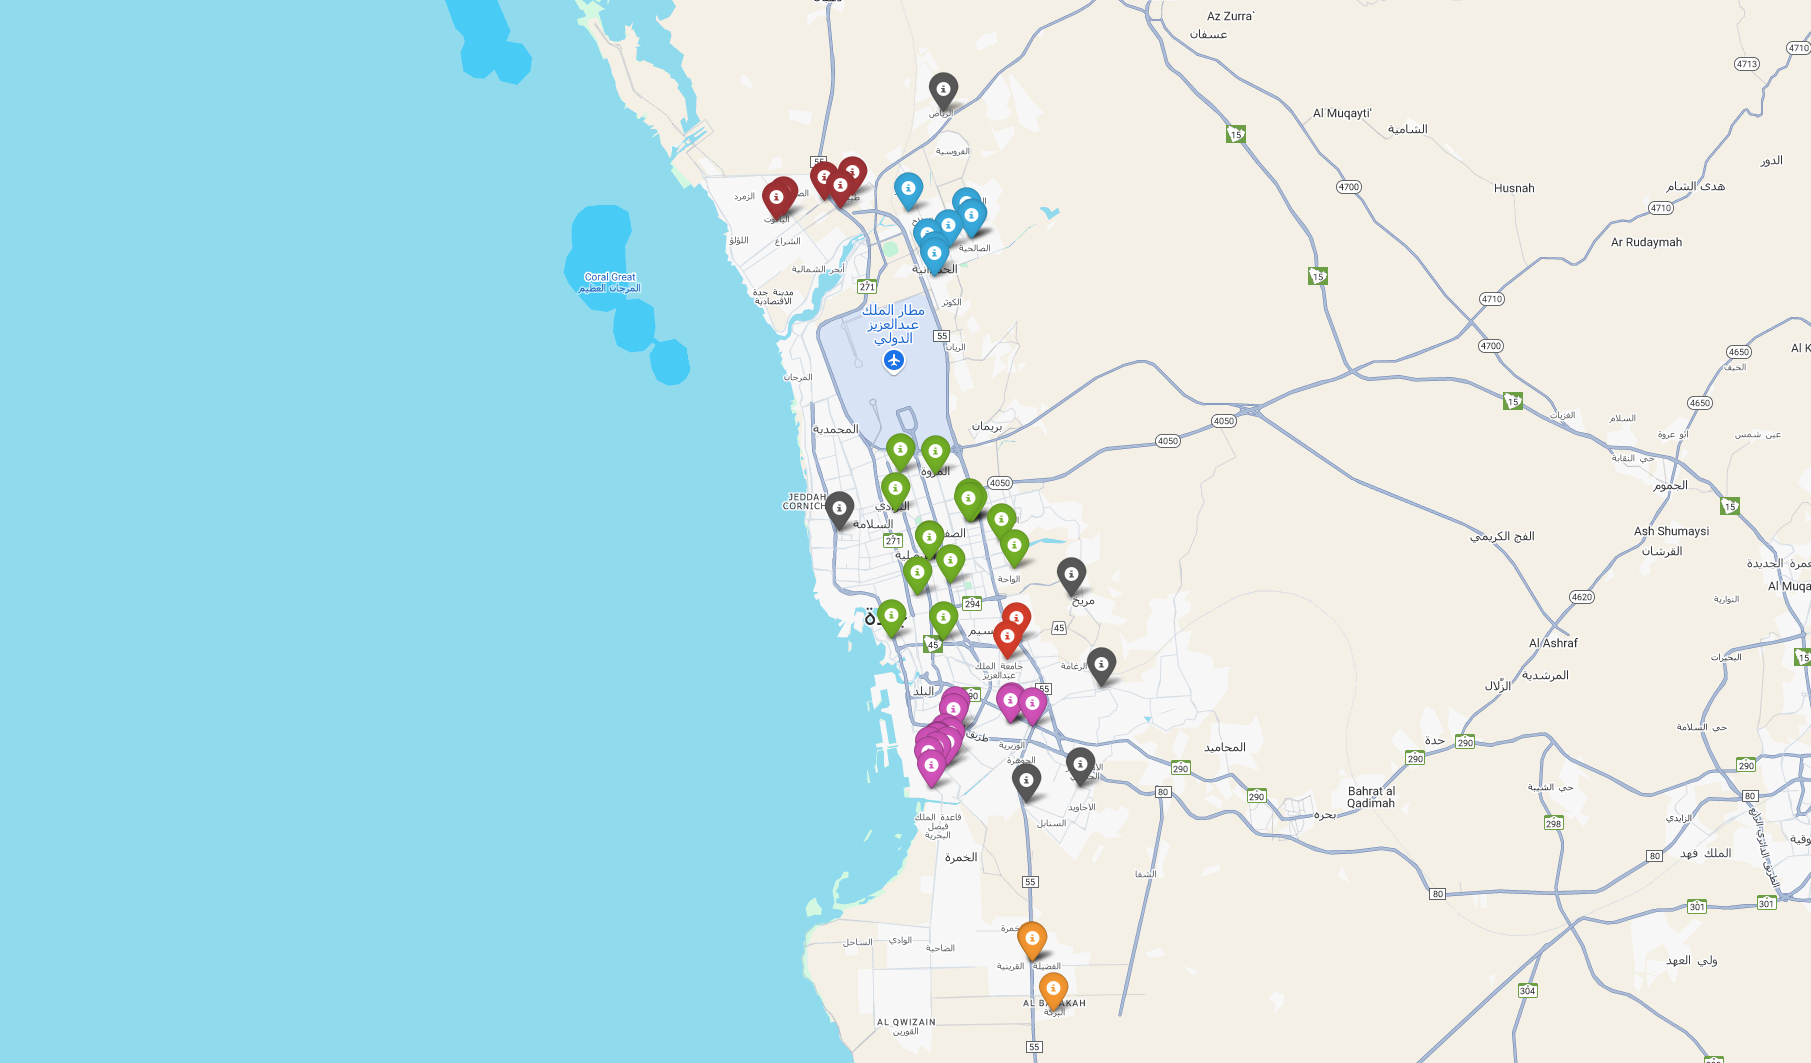
\includegraphics[width=\textwidth]{gfx/map_clusters.png}
    \caption{Cluster mapping based on customer locations}
    \label{fig:map_clusters}
\end{figure}
% After fetching the orders and invoices, the DBSCAN algorithm will cluster the customers based on their locations as shown in Figure \ref{fig:map_clusters}.
Once the orders and invoices are retrieved, the DBSCAN algorithm is applied to group customers according to their locations, as illustrated in Figure \ref{fig:map_clusters}.
\newpage

\begin{figure}[htbp]
    \centering
    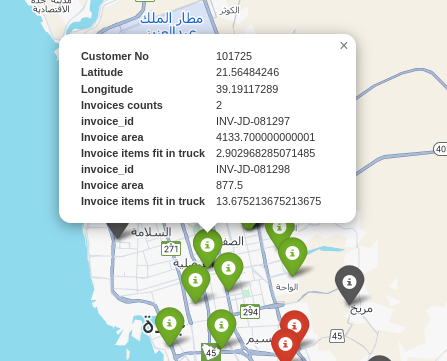
\includegraphics[width=\textwidth]{gfx/customer_map.png}
    \caption{Customer details}
    \label{fig:cutomer_info}
\end{figure}
Each cluster has multiple customer locations with their orders. Then, the order sizes will be calculated to determine how many trucks are needed and the appropriate truck sizes as shown in Figure \ref{fig:cutomer_info}.

\newpage
\subsection{Template 2: Vehicle Routing Problem(VRP) Summary}

\begin{figure}[htbp]
    \centering
    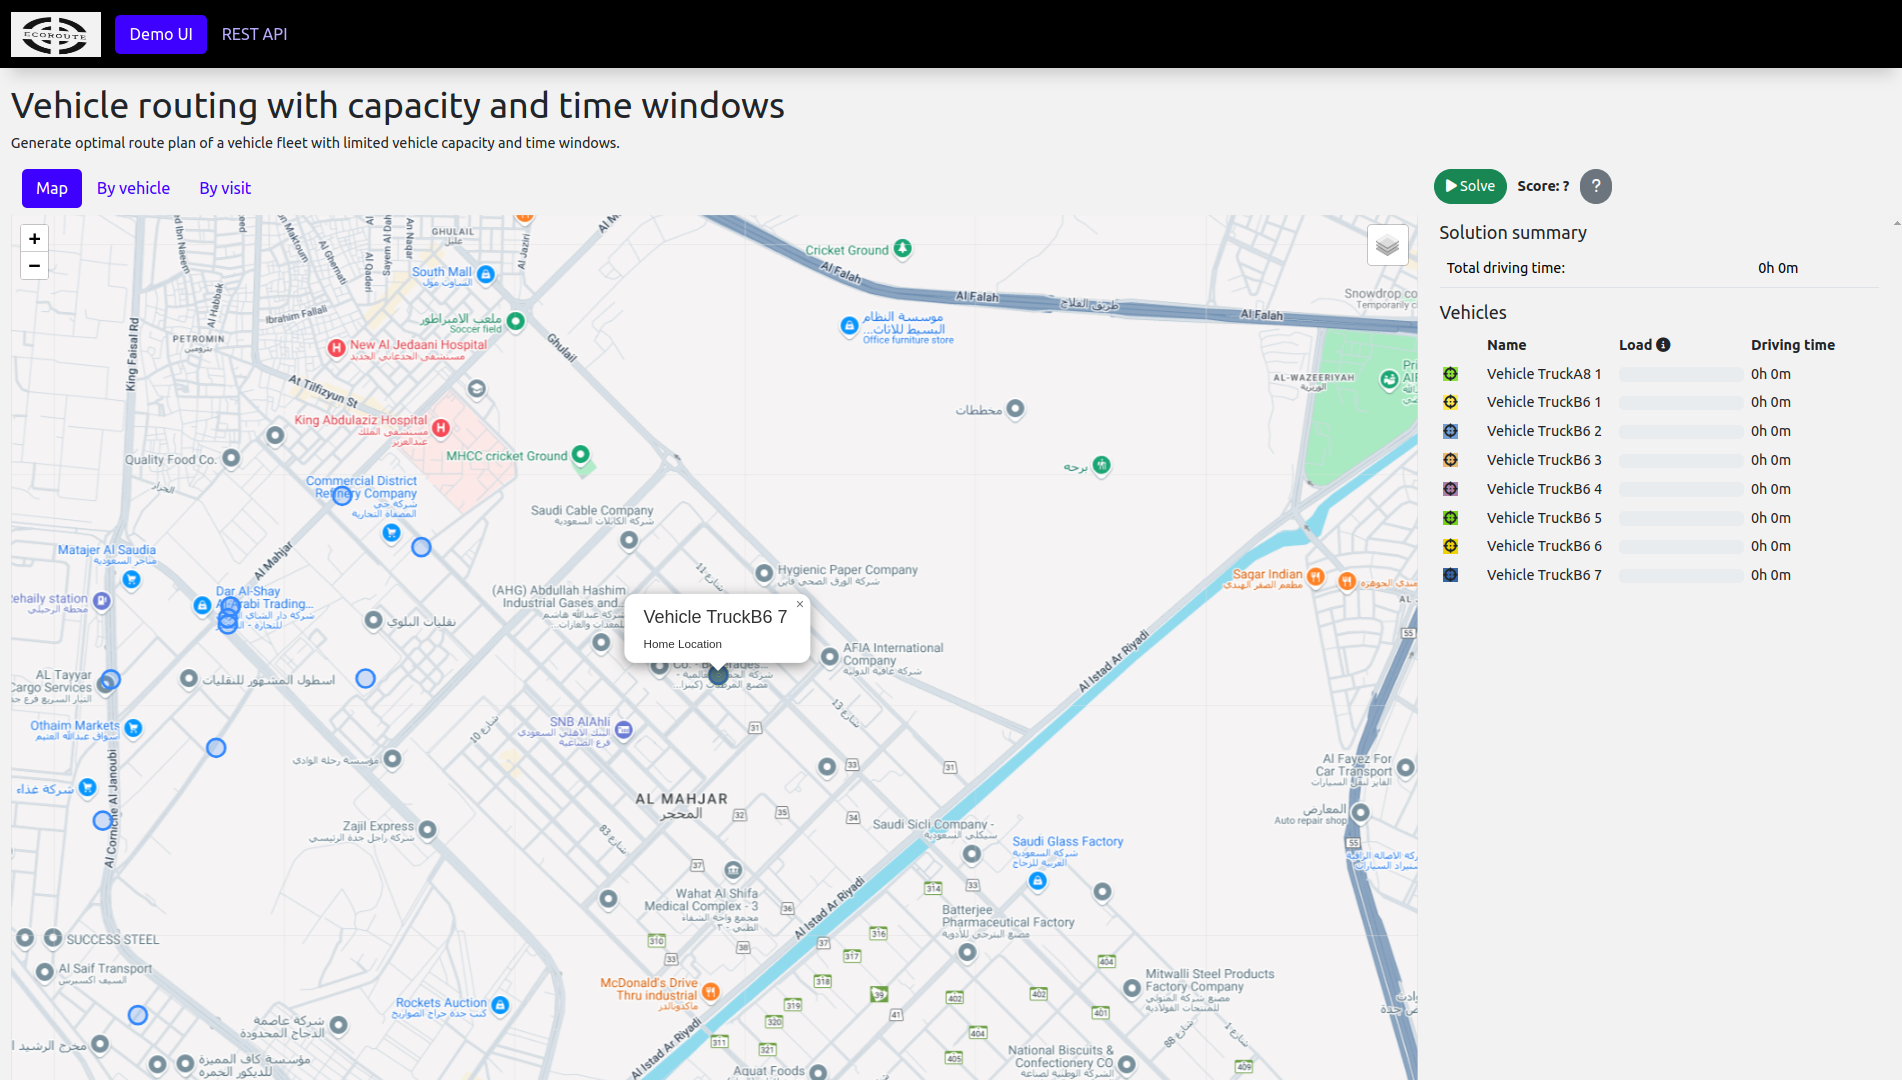
\includegraphics[width=\textwidth]{gfx/VRP_1.png}
    \caption{Location of the truck departure center}
    \label{fig:VRP_1}
\end{figure}

This is the location of the truck departure center as shown in Figure \ref{fig:VRP_1}.
\newpage
\begin{figure}[htbp]
    \centering
    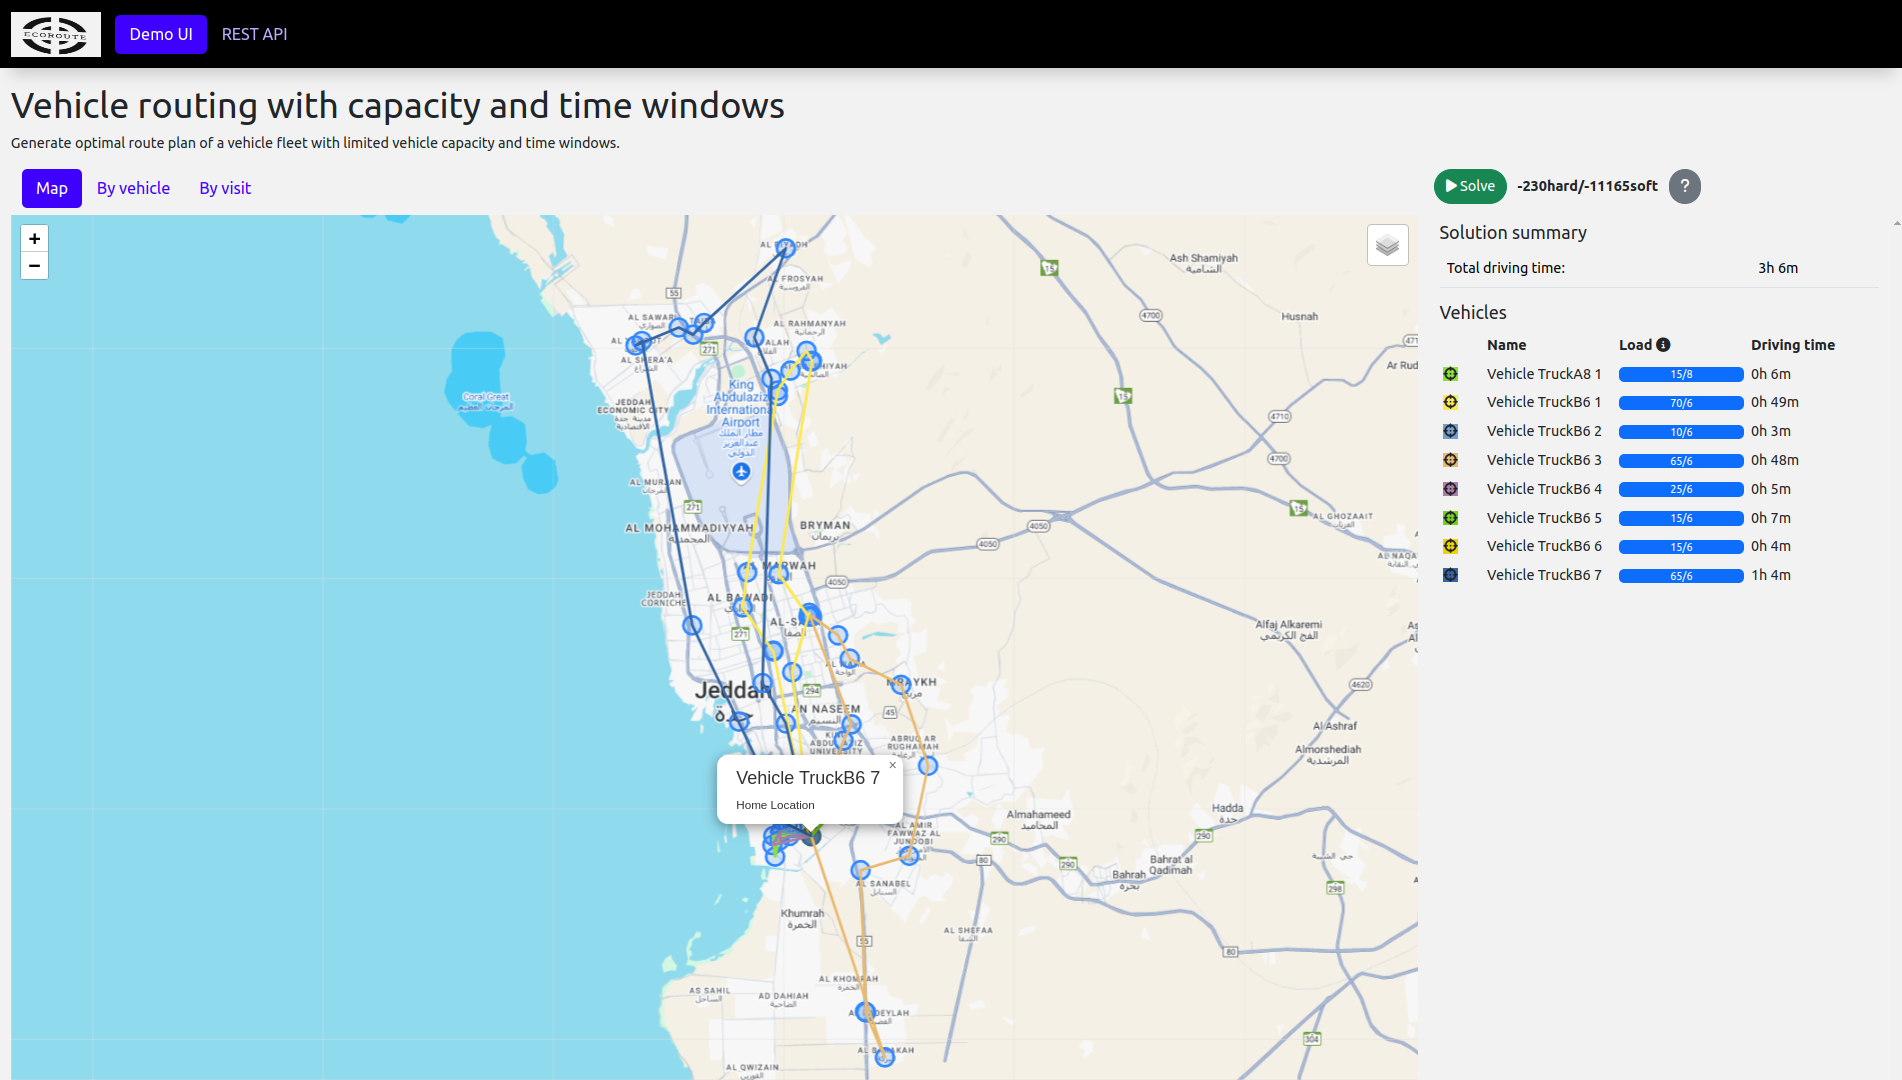
\includegraphics[width=\textwidth]{gfx/VRP_2.png}
    \caption{Vehicle Routing}
    \label{fig:VRP_2}
\end{figure}

The following explains Figure \ref{fig:VRP_2}.
\begin{itemize}
    
    \item \textbf{Map Visualization}: The map on the left side shows the routing paths of several vehicles as they navigate through a geographical region. It includes:
        \begin{itemize}
            \item Multiple colored lines represent the routes taken by each vehicle.
            \item Markers indicating stops or delivery points, which are likely part of the optimization problem.
            \item The routes appear optimized for minimizing distance and delivery time based on capacity and time constraints.
        \end{itemize}

    \item \textbf{Solution Summary Panel (Right Side)}:
        \begin{itemize}
        \item Total Driving Time: The total driving time for all vehicles in the fleet is 3 hours and 6 minutes.
        \item Vehicle List: The panel provides details for each truck involved in the delivery process:
        \item Vehicle Names: Each vehicle is labeled (e.g., Vehicle TruckA, TruckB).
        \item Load (\%): Indicates the percentage of each vehicle’s capacity that is being utilized. For example, TruckA is only utilizing 1.5\% of its capacity, whereas TruckB6 is using 66%.
        \item Driving Time: Shows the time spent driving for each vehicle, ranging from a few minutes to over an hour (e.g., Vehicle TruckB6 has been driving for 1 hour and 4 minutes).
    \end{itemize}

    \item \textbf{Legend and Options}:
        \begin{itemize}
            \item There’s an option labeled "Solve" that allows recalculating or solving the routing problem under current constraints.

            \item The title emphasizes that the routing is optimized for limited vehicle capacity and time windows.
        \end{itemize}

\end{itemize}
\newpage

\begin{figure}[htbp]
    \centering
    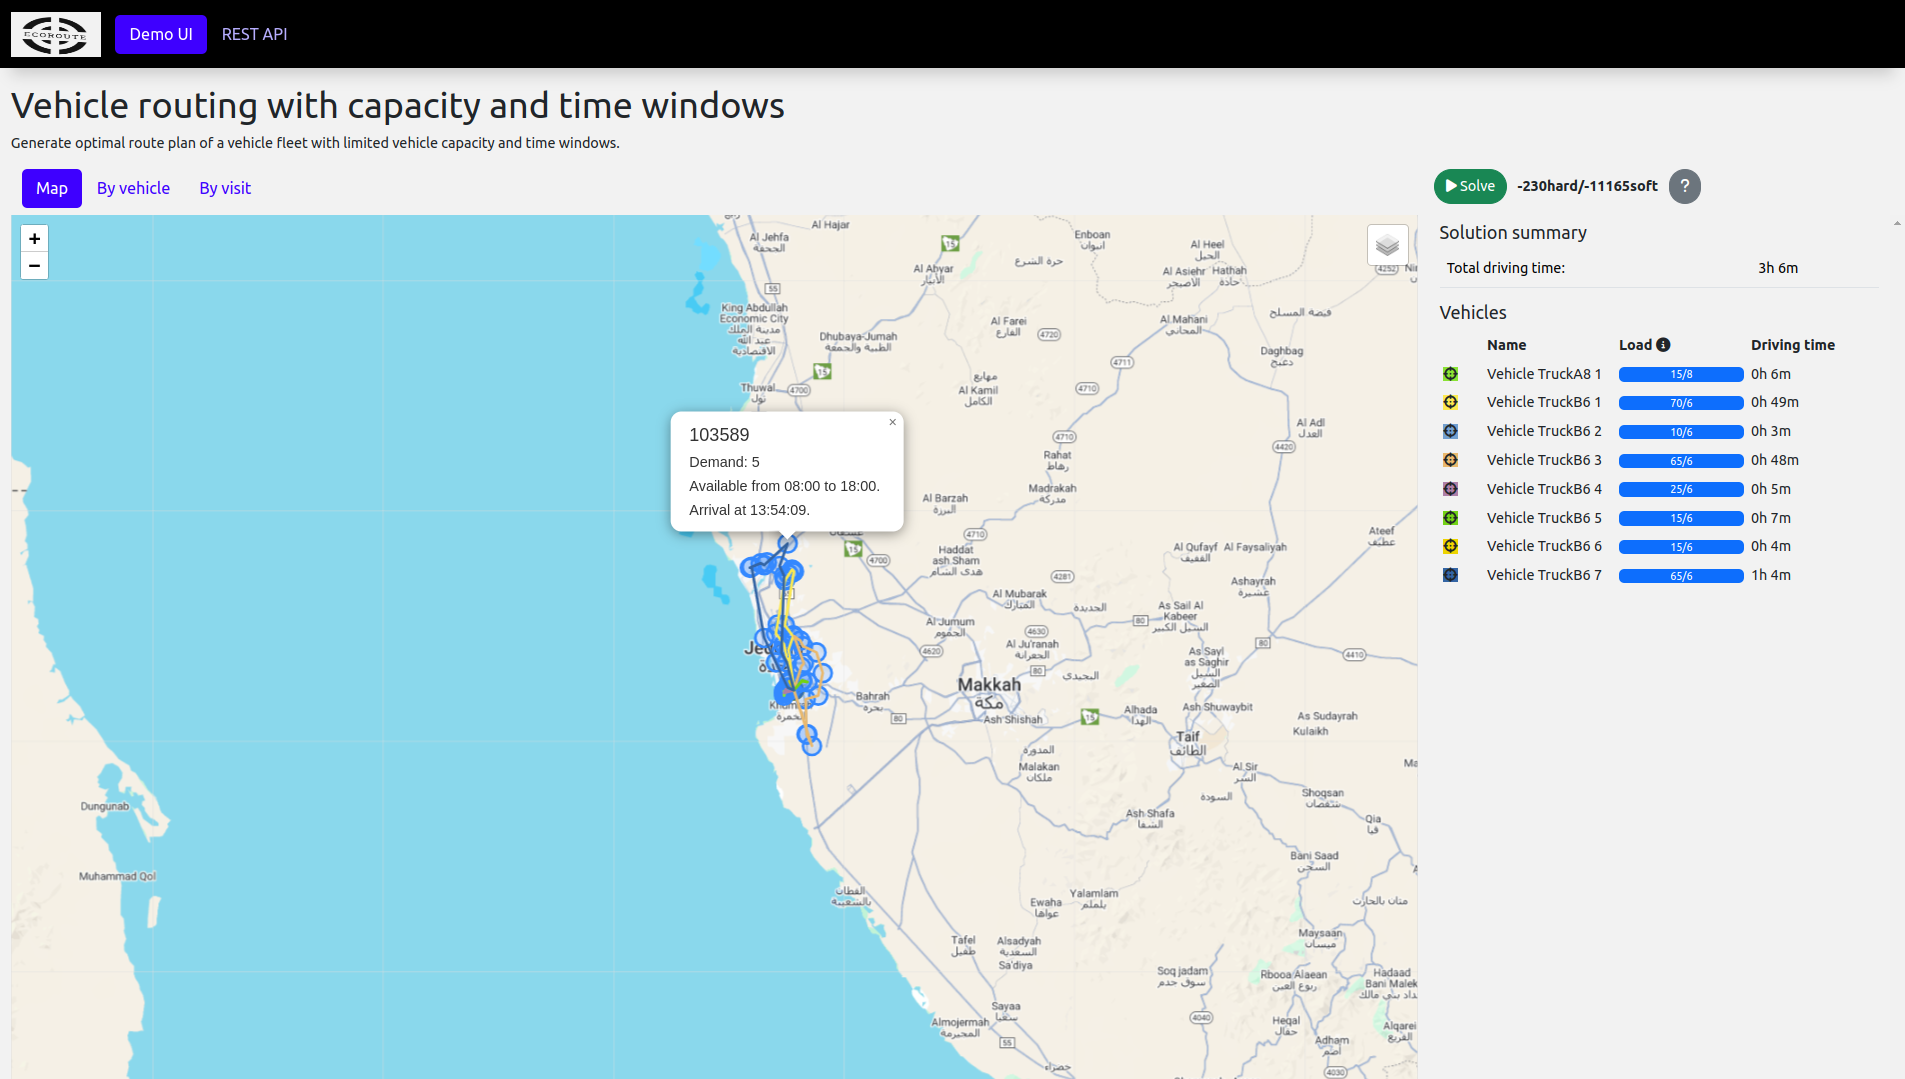
\includegraphics[width=\textwidth]{gfx/VRP_3.png}
    \caption{Customer details}
    \label{fig:VRP_3}
\end{figure}
This map displays the customer's location along with details about their availability, including opening and closing hours, as shown in Figure \ref{fig:VRP_3}.
\newpage


\begin{figure}[htbp]
    \centering
    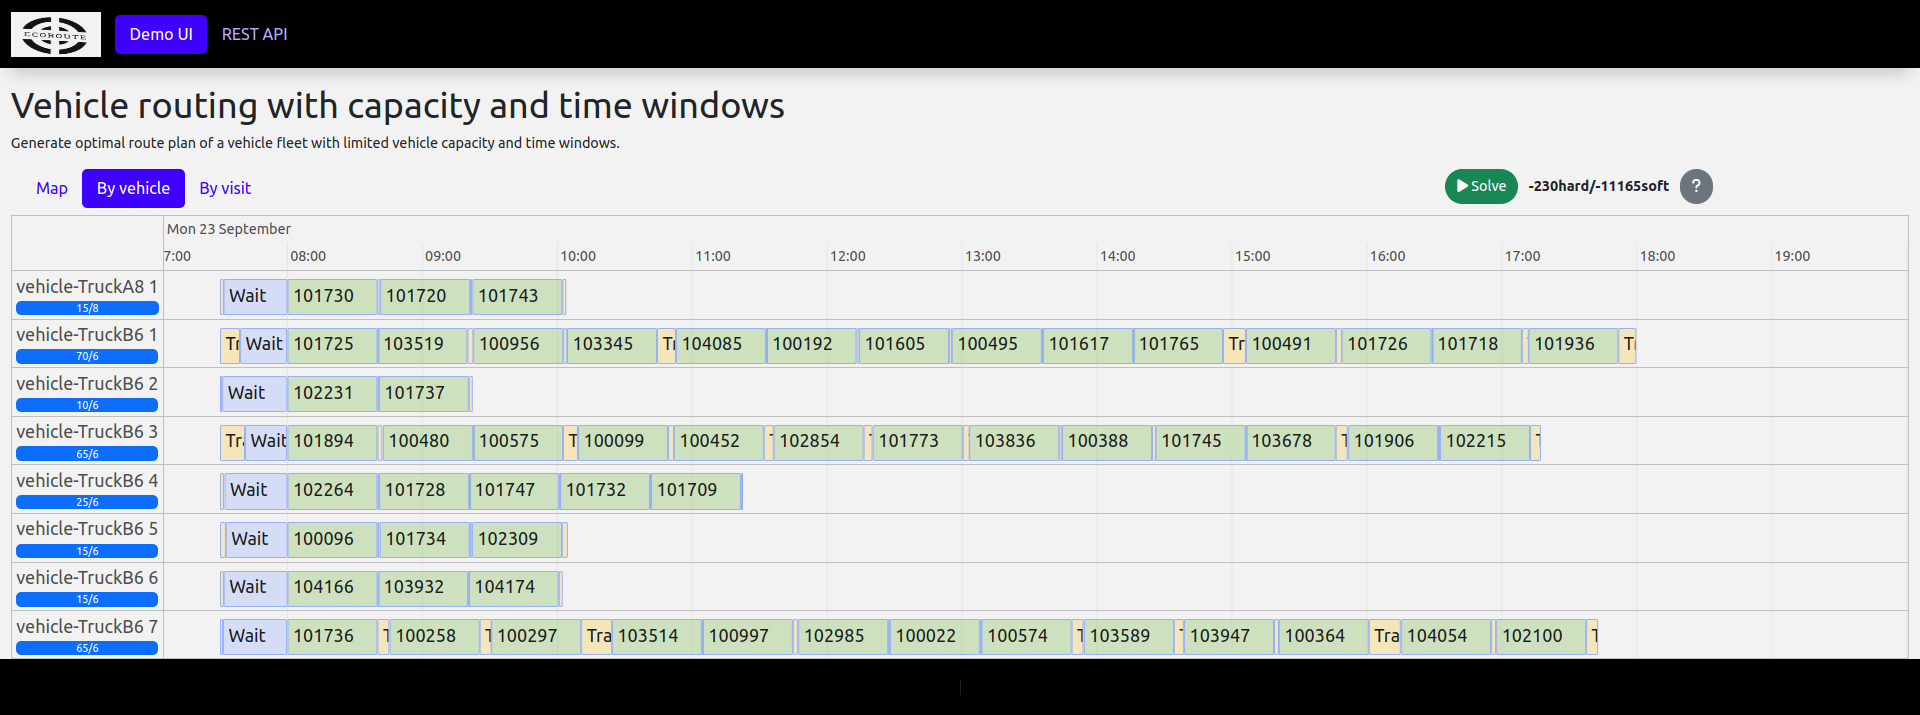
\includegraphics[width=\textwidth]{gfx/VRP_4.png}
    \caption{By Vehicle}
    \label{fig:VRP_4}
\end{figure}
The following explains Figure \ref{fig:VRP_4}.
\begin{itemize}
    \item \textbf{Title and Description}:
        \begin{itemize}
            \item The title specifies that this is a vehicle routing with capacity and time windows, designed to generate an optimal route plan for a fleet of vehicles with these constraints.
            \item There are tabs to switch between viewing the map or analyzing the data "By Vehicle" or "By Visit." The current view is set to "By Vehicle."
        \end{itemize}
    \item \textbf{Time Axis (Top)}:
        \begin{itemize}
            \item The chart covers a full day, starting from 7:00 AM to 7:00 PM, broken down by hours. Each vehicle’s schedule is displayed horizontally across this time period.
        \end{itemize}
    \item \textbf{Vehicle Schedule (Left)}:
    \begin{itemize}
        \item On the left side, there are labels for each truck involved in the routing process (e.g., Vehicle TruckA1, Vehicle TruckB6).
        \item Next to each vehicle's name is its capacity usagein percentage, such as:
            \begin{itemize}
                \item Truck A1: 1.5\%
                \item Truck B6: 70\%
                \item Truck B7: 66\%
            \end{itemize}
    \end{itemize}
\end{itemize}
\newpage

\begin{figure}[htbp]
    \centering
    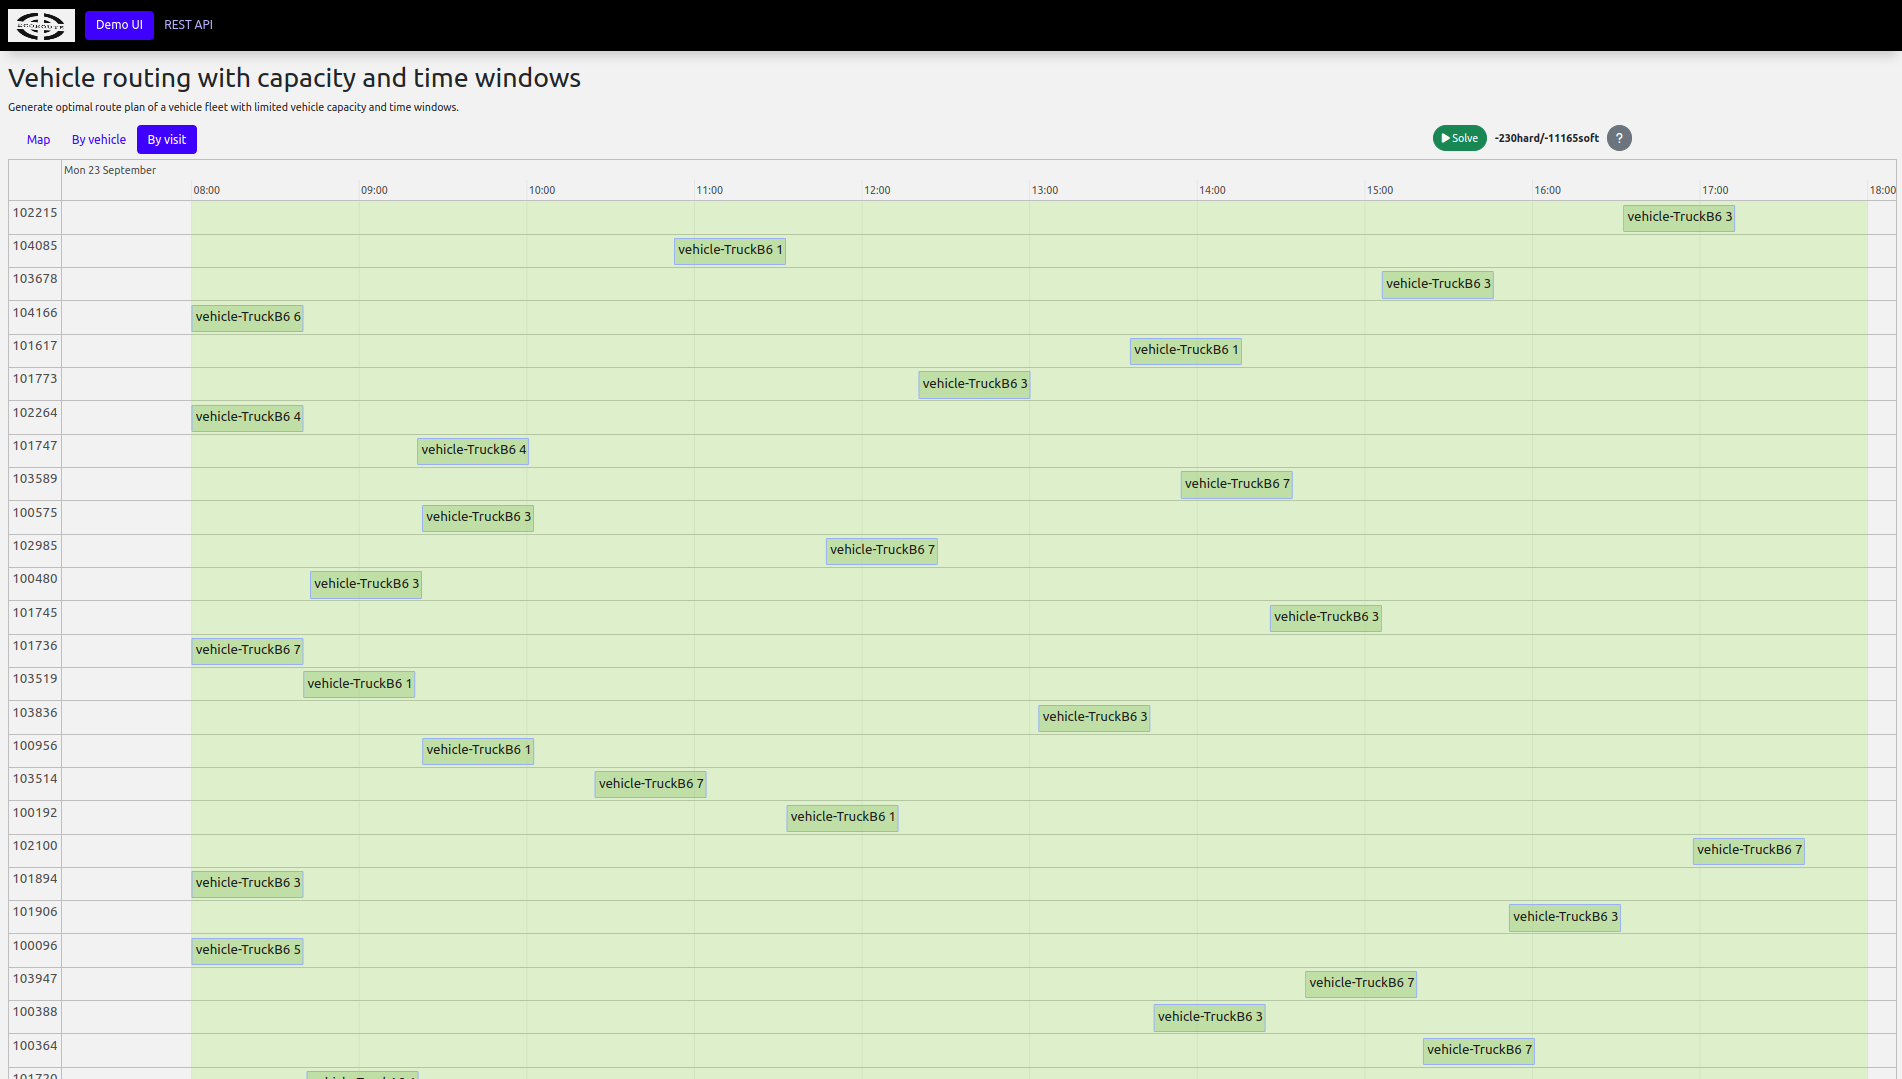
\includegraphics[width=\textwidth]{gfx/VRP_5.png}
    \caption{By Visit}
    \label{fig:VRP_5}
\end{figure}

The following explains Figure \ref{fig:VRP_5}.
\begin{itemize}

    \item \textbf{Title and Overview}:
        \begin{itemize}
            \item   The view selected is "By Visit", indicating that each row in the chart corresponds to a specific visit or delivery stop.
    \end{itemize}

\item \textbf{Time Axis (Top)}:
    \begin{itemize}
        \item The time axis runs from 07:00 AM to 6:00 PM, covering the operational hours during which deliveries are scheduled.
        \item Each visit is plotted on this timeline, showing when the visit occurs and which vehicle is responsible for that visit.
    \end{itemize}
\item \textbf{List of Visits (Left)}:
    \begin{itemize}
        \item The left side shows visit IDs (e.g., 102215, 100495, 101717) which represent delivery or pickup locations.
        \item Each row corresponds to a specific visit, indicating the truck assigned to that visit.
    \end{itemize}
\item \textbf{Vehicle Assignments (Main Grid)}:
    \begin{itemize}
        \item The grid shows the assignments of specific vehicles to visits at particular times.
        \item Each green cell contains the name of a vehicle (e.g., vehicle-TruckB6 1, vehicle-TruckB7 1), indicating which truck is handling a specific delivery.
        \item The horizontal placement of the vehicle name indicates the scheduled time for that visit.
        \item The vertical alignment shows the relationship between the different visits that the same vehicle handles.
    \end{itemize}
\end{itemize}
\newpage
\begin{figure}[H]
    \centering
    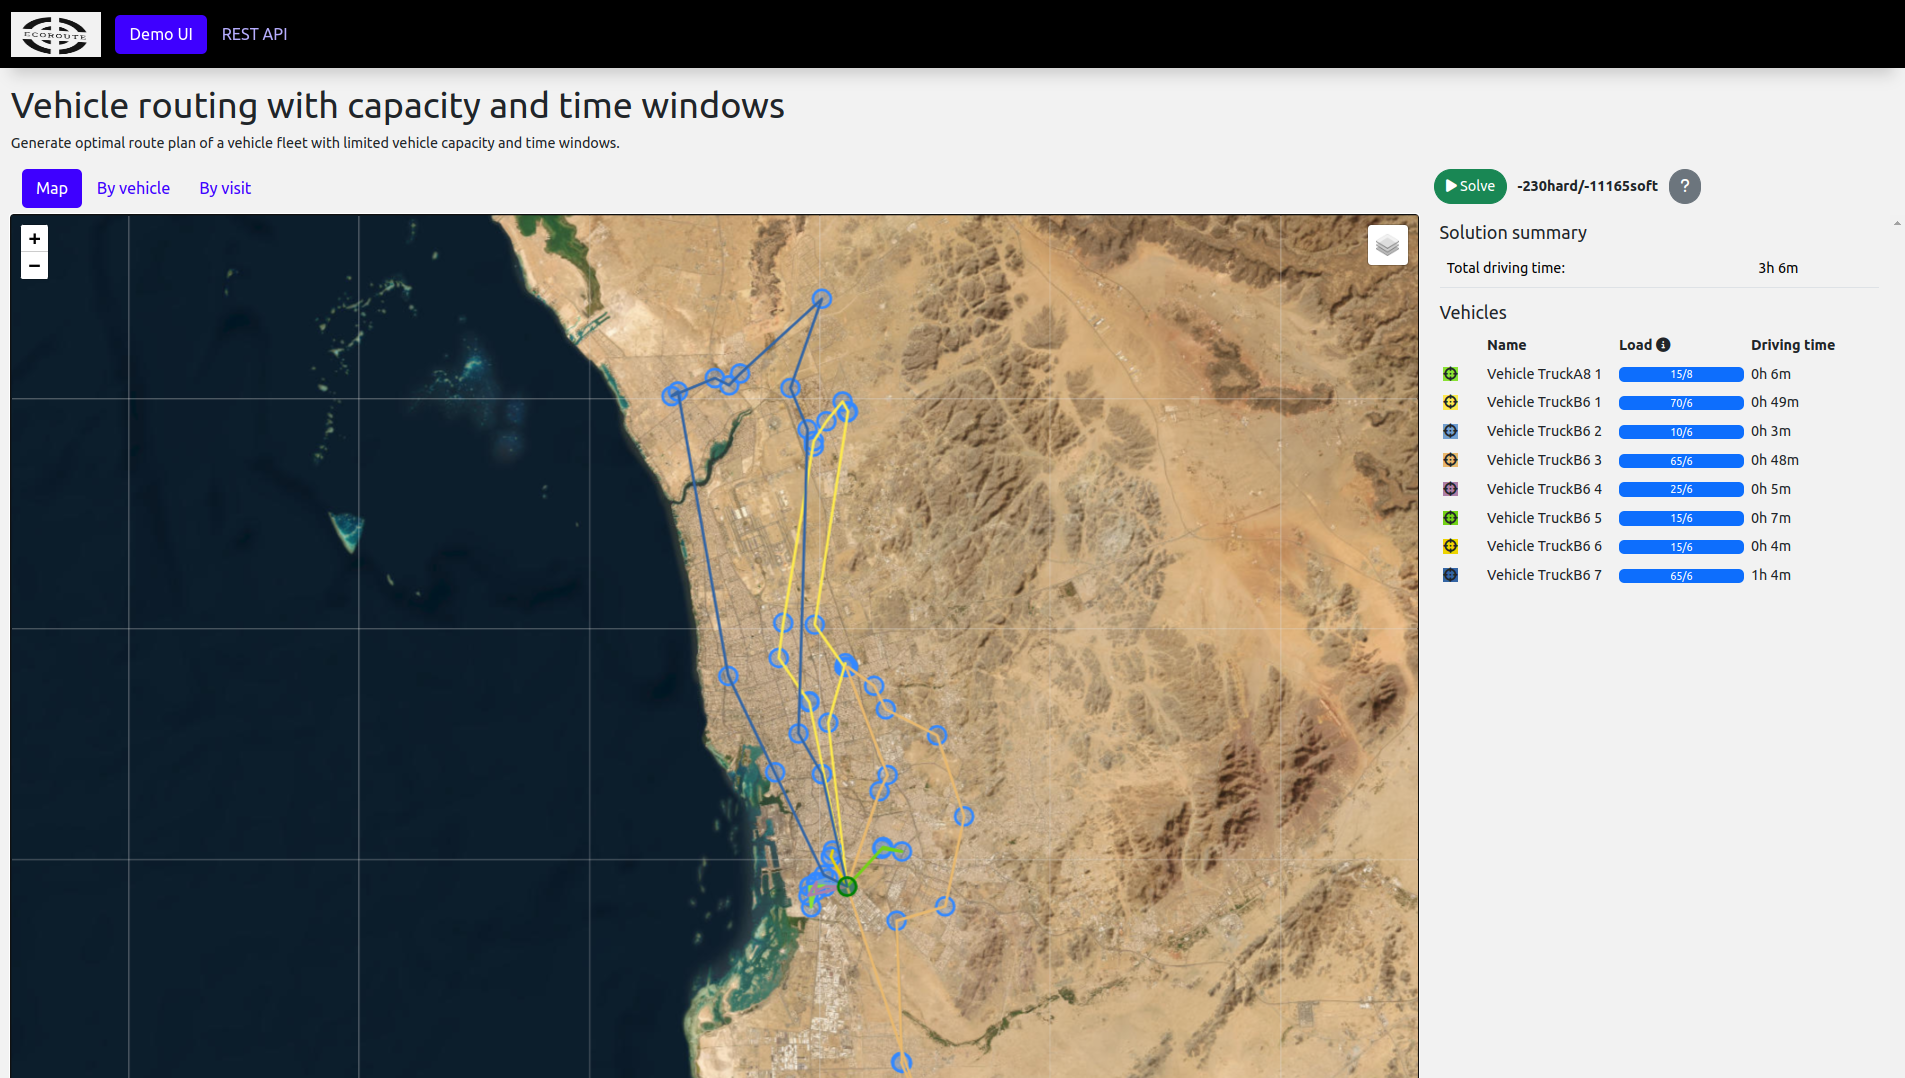
\includegraphics[width=\textwidth]{gfx/VRP_6.png}
    \caption{Esri map}
    \label{fig:VRP_6}
\end{figure}

\begin{figure}[H]
    \centering
    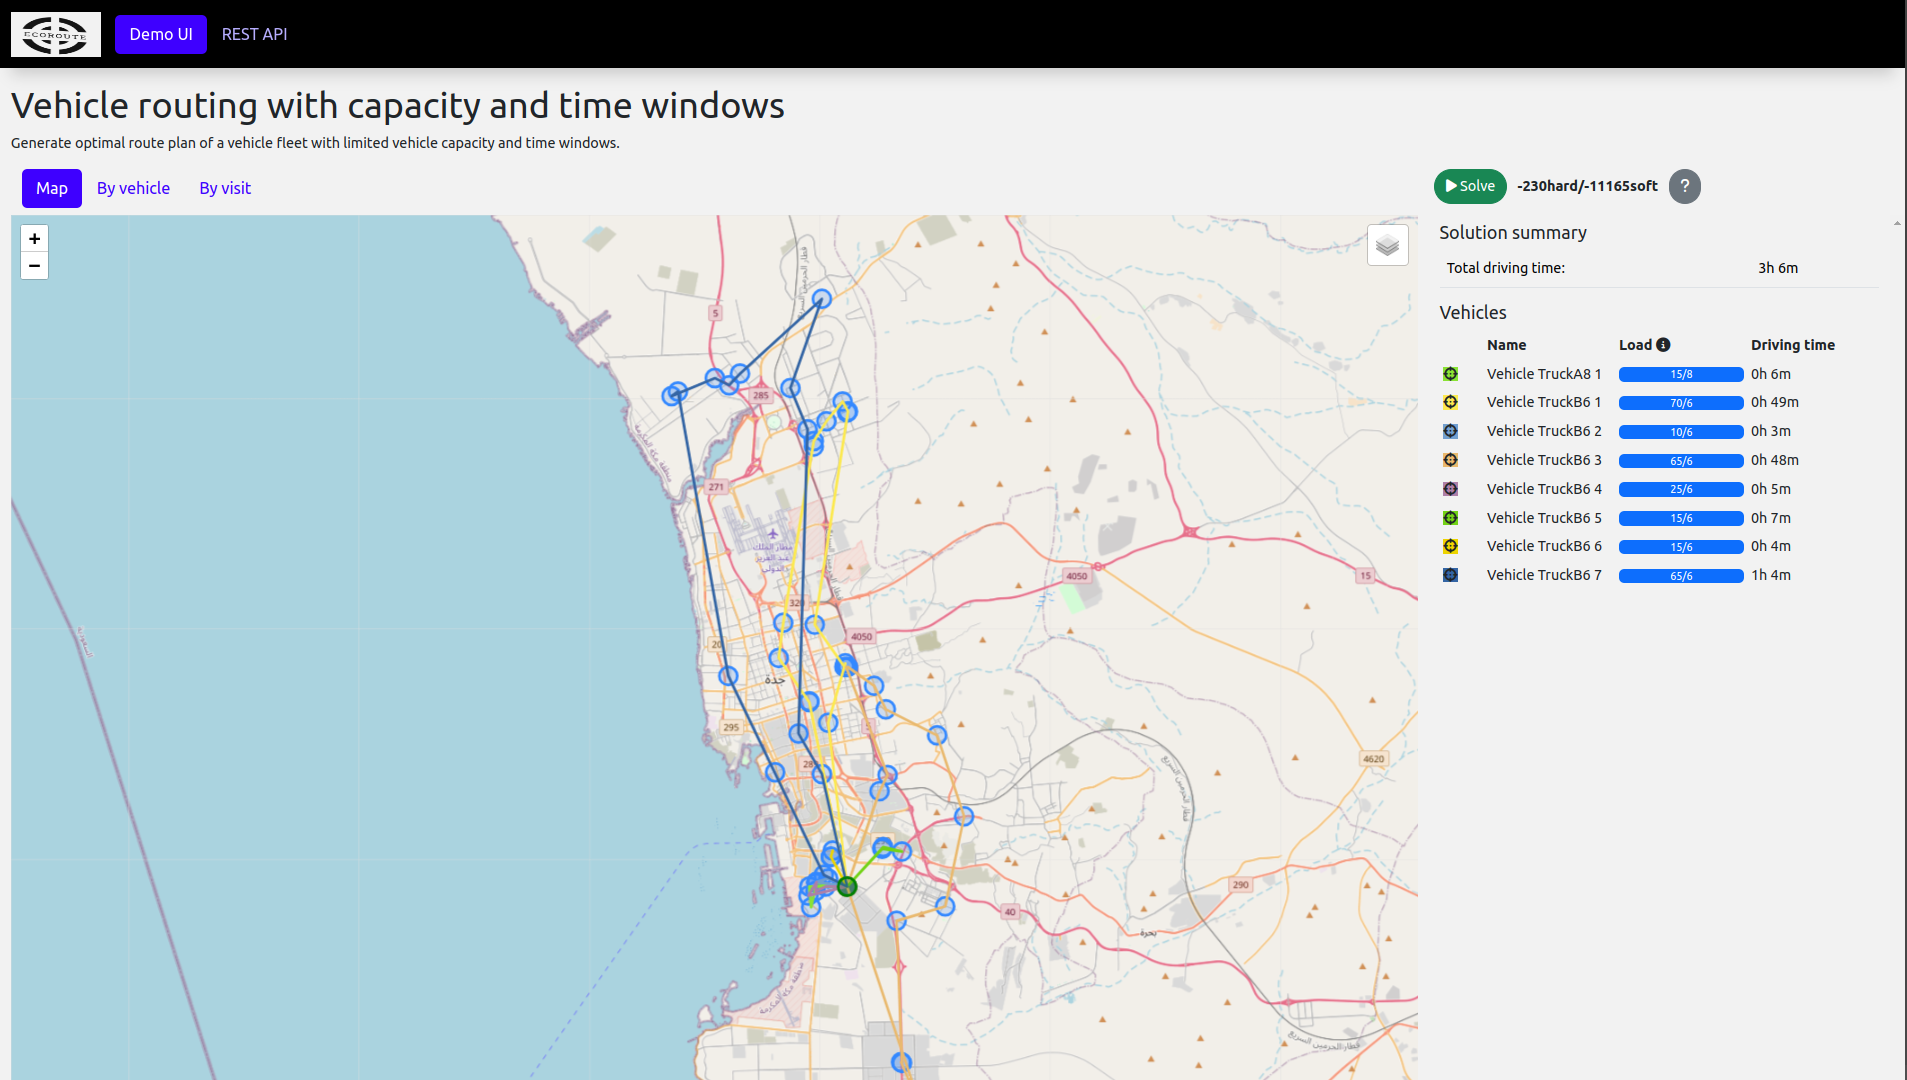
\includegraphics[width=\textwidth]{gfx/VRP_7.png}
    \caption{OpenStreetMap}
    \label{fig:VRP_7}
\end{figure}

We support OpenStreetMap and Esri maps, as shown in Figures \ref{fig:VRP_6} and \ref{fig:VRP_7}.
\newpage

\section{Algorithms}
The following algorithms are integral to the system:
\begin{enumerate}
    \item \textbf{DBSCAN/K-means}: For clustering customers based on their geographic proximity.
    \item \textbf{Google OR-Tools}: Solving the Vehicle Routing Problem.
    \item \textbf{Simulated Annealing}: Used for route optimization when handling larger datasets.
\end{enumerate}

\section{Technologies}
\begin{itemize}
    \item \textbf{Languages}: Java, Python, Javascript, HTML, CSS, SQL for database management.
    \item \textbf{Programming libraries}:  FastAPI, Pandas, sklearn, folium, numpy, timefold, OR-Tools, leaflet, timeline, vis-timeline.
    \item \textbf{Framework}: Bootstrap. 
    \item \textbf{APIs}: Google Maps API for route data, OR-Tools for solving optimization problems.
    \item \textbf{Database}: SQL database for customer and delivery data.
    \item \textbf{Maps}: OpenStreetMap, Google maps, Esri.
    \item \textbf{Version control}: git/github.
\end{itemize}

\section{System Integration}
\subsection{API Integration Approach}
\begin{itemize}
    \item \textbf{Data Exchange Format}: All data will be exchanged in JSON format to ensure compatibility and ease of use across different systems. JSON is lightweight and widely supported, making it ideal for integration.
    \item \textbf{API Functions}: Data Fetching API: This API will pull customer orders, delivery addresses, and other relevant information from the OMS and CRM systems. It will validate the data and format it as required for clustering and routing algorithms.
    \item \textbf{Data Processing API}: After processing the input data (clustering and route optimization), this API will return the optimized routes, truck assignments, and delivery schedules in JSON format to the logistics management system.
    \item \textbf{Status Update API}: This API will allow real-time updates on delivery status, delays, or any changes in route to be sent back to the OMS and CRM systems. This will help keep all stakeholders informed and improve customer service.
    \item \textbf{Integration Steps}:
        \begin{enumerate}
            \item Develop APIs to extract data from existing systems, ensuring all necessary information is available for clustering and route optimization.
            \item Implement the clustering and routing algorithms to process the data and generate optimized routes.
            \item Develop APIs to return the optimized routes and truck assignments to the logistics management system.
            \item Implement real-time update APIs to keep track of delivery status and communicate any changes back to the relevant systems.
        \end{enumerate}

    \item \textbf{Security and Data Privacy}:All API calls will be secured using HTTPS, with authentication tokens to ensure data security and integrity.
        Sensitive customer data will be encrypted, and access will be restricted to authorized personnel only, in compliance with data protection regulations (e.g., GDPR).

\end{itemize}

\section{Strategy}
\begin{itemize}
    \item \textbf{Training}: Staff will undergo training on using the new system for route management.
    \item \textbf{Integration}: Incorporate AI systems to continuously improve route optimization based on real-time data and historical trends.
    \item \textbf{Optimization}: Regularly review and refine clustering and routing models.
\end{itemize}


\section{Potential Risks and Mitigation}
There may be resistance to change from staff. To mitigate this, training sessions should be provided
to explain the benefits and how to use the new system.

\section{Future Plan}
\begin{itemize}
\item The future plan involves integrating more AI/ML/DL models to dynamically adjust routes in real time and predict traffic conditions. As the number of customers grows, the system will scale using cloud computing services (e.g., AWS, Azure, Google Cloud).
\item \textbf{Customer App}: Allows customers to view their delivery status, estimated time of arrival, and the route being taken.
\item \textbf{Driver's Vehicle App}: Provides real-time route updates, delivery instructions, and traffic alerts using GPS and AI predictions
\end{itemize}



\section{Conclusion}
Optimizing truck routing will help reduce costs and improve operational efficiency. We encourage
the company to adopt this solution and move forward with further discussions in an upcoming
meeting.





% End Document
\end{document}
